\documentclass[letterpaper]{article} % DO NOT CHANGE THIS
\usepackage{aaai2027}  % DO NOT CHANGE THIS
\usepackage[hyphens]{url}  % DO NOT CHANGE THIS
\usepackage{graphicx} % DO NOT CHANGE THIS
\urlstyle{rm} % DO NOT CHANGE THIS
\def\UrlFont{\rm}  % DO NOT CHANGE THIS
\usepackage{natbib}  % DO NOT CHANGE THIS AND DO NOT ADD ANY OPTIONS TO IT
\usepackage{caption} % DO NOT CHANGE THIS AND DO NOT ADD ANY OPTIONS TO IT
\frenchspacing  % DO NOT CHANGE THIS
\usepackage{booktabs}
\usepackage{amsfonts}
\usepackage{amsmath}
\graphicspath{{../figs/}}
\usepackage{xr}
\externaldocument{main}
\renewcommand{\thefigure}{A\arabic{figure}}
\renewcommand{\thetable}{A\arabic{table}}
\pdfinfo{
/TemplateVersion (2027.1)
}
\setcounter{secnumdepth}{0}

\title{Black--Scholes for the Land:\\ Modelling Savannah Response to Rain as a Dynamic World Model\\ Appendix}
\author{
    Tom Pitts
}
\affiliations{
    AFFILIATION TO CONFIRM\\
    tom.d.pitts@gmail.com
}

\begin{document}
\maketitle

\section{Location, Data, Tables, Calibration, Fitting}
\paragraph{Data and preparation} Three sources are fused onto one grid and one calendar. The surface is MODIS Terra MOD13Q1 v061 NDVI \citep{mod13} at $250$\,m, one composite per 16 days from 2002 to 2025 (537 composites), warped to a $0.0025^\circ$ grid of $160\times160$ pixels per box. Pixels whose reliability flag exceeds 1 (cloud, snow, fill; $2\%$ of pixel-steps) are treated as unobserved: their values are interpolated in time so the model always has an input state, but they are never used as targets. Each pixel's climatology is its mean NDVI per composite-of-year over 2003--2018, and the anomaly $a_t$ is NDVI minus that climatology. The driver is CHIRPS v2 daily rainfall \citep{chirps} at $0.05^\circ$, summed over each composite's 16-day window and bilinearly resampled to the grid, in units of $100$\,mm, with a climatology built the same way. Static covariates $x$ are the pixel's mean NDVI, seasonal amplitude and climatological annual rain. MCD64A1 burned area \citep{mcd64} gives the day each $500$\,m cell burned, and a pixel is marked burned in the composite window containing that day. The MODIS record has gaps: no composites for 61 days after 1 November 2021, so October--December 2021, one of the two drought seasons, contributes two composites, and about 30 days after 2 February 2023, 27 July 2024 and 2 December 2024. Steps spanning a gap are not yet excluded from any analysis.

\paragraph{Residual runs} The residual and counterfactual of Figures~\ref{fig:attribution} and~\ref{fig:fire} use the fitted M2 with no refitting; each season starts from the observed state before its first 16-day window and runs six windows. The shaded range in Figure~\ref{fig:attribution} re-runs March--May 2022 along its observed rain 500 times, each step's residual a whole map drawn from the same step of a random March--May season in 2003--2017, which keeps the residual's spatial correlation. Re-injecting $\hat\varepsilon$ along the rain that fell reproduces the observed anomaly to a maximum absolute error of $10^{-6}$ in every season. Box-mean anomaly at three months for all 13 held-out seasons is in the supplementary run directory. The year-to-year persistence of the residual and its forecast value were tested with a per-pixel, per-year latent in the drift, inferred by MAP on one year and used to forecast the next: the latent beats a pixel-shuffled control on both boxes but improves three-month error by $0.3$--$0.6\%$, not significant on either. Residual against rain, held-out rainy-season pixel-steps: correlation $0.05$ ($0.03$ on training years); mean residual in spread units by rain departure, below $-60$\,mm / $-60$ to $-30$ / $-30$ to $0$ / $0$ to $30$ / $30$ to $60$ / $60$ to $120$ / above $120$\,mm: $-0.24$, $-0.03$, $-0.03$, $+0.22$, $+0.05$, $+0.10$, $-0.01$ on held-out years against $-0.04$, $+0.07$, $+0.12$, $+0.16$, $+0.13$, $+0.09$, $+0.20$ on training years. Fire, 17 January 2021 burn scored on the 2 February composite: mean residual on burned pixels $-0.75$ against $-0.04$ elsewhere; mean z-score $-0.17$ against $-0.13$.

\begin{figure*}[t]
\centering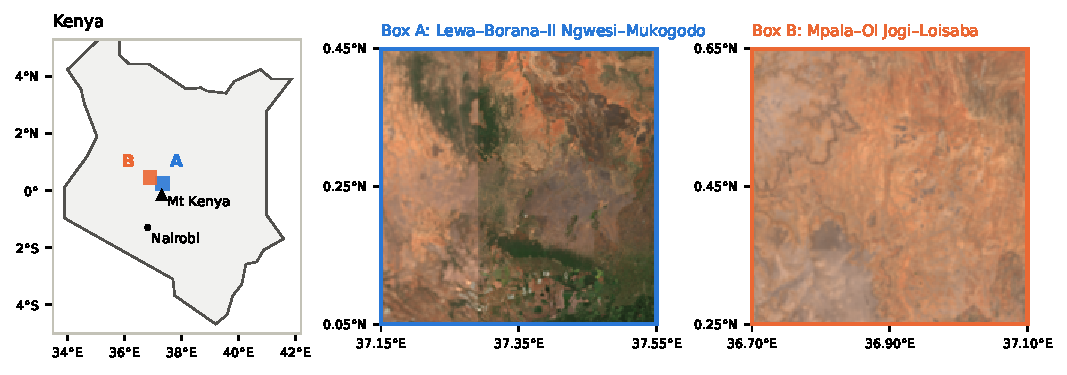
\includegraphics[width=\textwidth]{fig_map.pdf}
\caption{Where. Left: Kenya with the two $45$\,km boxes; Box A spans $37.15$--$37.55^\circ$E, $0.05$--$0.45^\circ$N, Box B $36.70$--$37.10^\circ$E, $0.25$--$0.65^\circ$N. Centre and right: Sentinel-2 true colour of each box in the 2023 dry season; dark green is forest and riverine woodland, pale is open rangeland. Contains modified Copernicus Sentinel data (2023).}
\label{fig:map}
\end{figure*}

\begin{table}[t]\centering\caption{One-step scores on observed held-out transitions. NLL is Gaussian negative log-likelihood per transition; skill is $1-\mathrm{CRPS}/\mathrm{CRPS}_{\mathrm{M0}}$.}\label{tab:onestep}\footnotesize\setlength{\tabcolsep}{1.5pt}
\begin{tabular}{lcccc}\toprule
 & \multicolumn{2}{c}{Box A, 2019--25} & \multicolumn{2}{c}{Box B, all years}\\
Model & NLL & CRPS skill & NLL & CRPS skill\\\midrule
M0 history only & -1.208 & 0.000 & -1.448 & 0.000\\
M1 linear, realised rain & -1.227 & 0.013 & -1.543 & 0.052\\
M1.5 S-curve, realised rain & -1.226 & 0.009 & -1.543 & 0.052\\
M2 without driver & -1.277 & 0.016 & -1.504 & 0.023\\
M2 learned, realised rain & -1.277 & 0.085 & -1.628 & 0.104\\
\bottomrule\end{tabular}\end{table}

\paragraph{Anomaly protocol} A pixel-step is flagged when its score exceeds a cutoff. The three scores (M2, M1, z-score) are on different scales, so each gets its own cutoff, set to flag $5\%$ of pixel-steps where nothing burned. With false alarms equalised, we ask what fraction of burned pixels each score flags within a month of the burn, and what fraction of pixel-steps it flags in the two drought seasons, when the land browned but nothing burned. This is a probe rather than a benchmark: one landscape, 208 burned pixel-composites, a score that flags only drops --- a variant adopted after the pre-registered two-sided score was run --- and one of the two drought seasons, October--December 2021, reduced to two composites by a gap in the MODIS record.

\begin{figure}[t]
\centering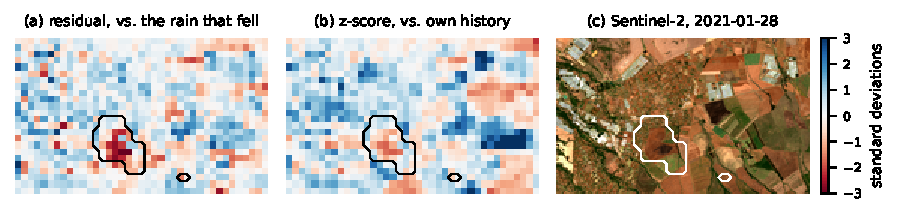
\includegraphics[width=\columnwidth]{fig_fire.pdf}
\caption{A burn on 17 January 2021 (outlined, 50 pixels), scored one composite later. (a) The residual of \eqref{eq:implied}: the burn is the red patch. (b) The z-score, the same composite against the pixel's own history: the burn is invisible. (c) Sentinel-2 true colour ten days after the burn: a harvested field on irrigated cropland, $80\%$ of the outline by area. Contains modified Copernicus Sentinel data (2021).}
\label{fig:fire}
\end{figure}

\begin{table*}[t]\centering\caption{Anomaly detection scored on fire, Box A 2019--25, 208 burned pixel-composites. Hit rate: burns flagged within two composites. Lag: mean composites from burn to flag among hits. FAR: unburned pixel-steps flagged in October--December 2021 and March--May 2022. AUC: rank separation of burns from unburned pixel-steps. Upper block: pre-registered two-sided score; lower block: one-sided drop score, post hoc.}\label{tab:anomaly}\small
\begin{tabular}{llcccc}\toprule
 & Score & hit rate @5\% FAR & lag (steps) & FAR, drought seasons & AUC\\\midrule
two-sided, pre-reg. & z-score & 0.06 & 0.54 & 0.017 & 0.558\\
 & M1 & 0.19 & 0.23 & 0.060 & 0.713\\
 & M1.5 & 0.19 & 0.23 & 0.061 & 0.710\\
 & M2 & 0.19 & 0.28 & 0.018 & 0.735\\
\midrule
one-sided, post hoc & z-score & 0.15 & 0.45 & 0.244 & 0.755\\
 & M1 & 0.27 & 0.25 & 0.148 & 0.711\\
 & M1.5 & 0.27 & 0.25 & 0.146 & 0.705\\
 & M2 & 0.28 & 0.24 & 0.051 & 0.773\\
\bottomrule\end{tabular}\end{table*}

\begin{figure}[t]
\centering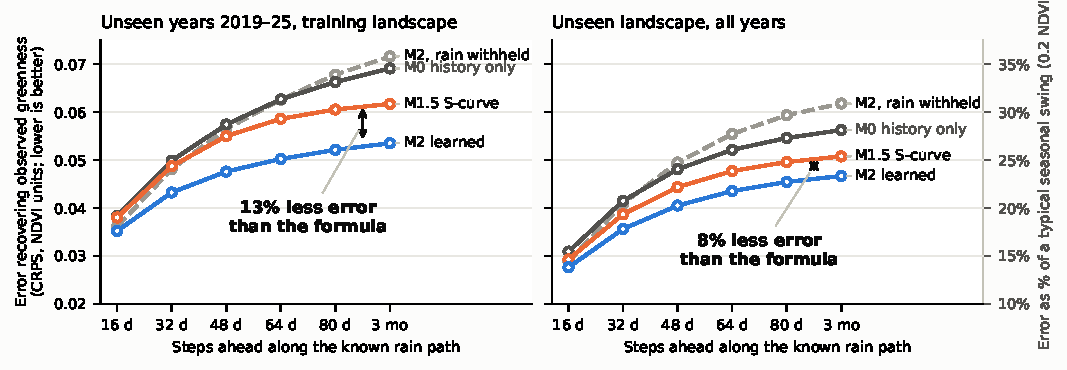
\includegraphics[width=\columnwidth]{fig2_response.pdf}
\caption{Given the rain that fell, how well does each model recover what the land did? CRPS of sampled rollouts against the observed anomaly along the known rain path; no model uses a rain forecast. Grey dashed: M2 fed climatological rain. Right axis: error as a share of a typical $0.2$ NDVI seasonal swing.}
\label{fig:response}
\end{figure}

\begin{figure}[t]
\centering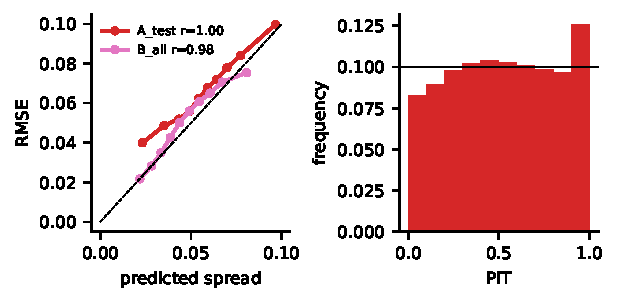
\includegraphics[width=\columnwidth]{fig3_calibration.pdf}
\caption{M2 calibration on held-out sets: RMSE against predicted spread by decile, and the PIT histogram \citep{gneiting2007b} on Box A 2019--25.}
\end{figure}

\begin{figure*}[t]
\centering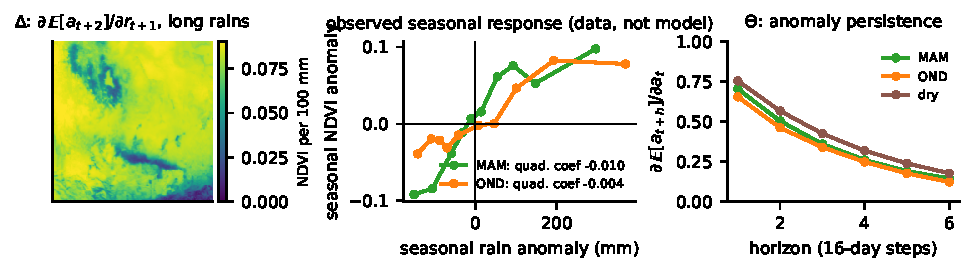
\includegraphics[width=0.96\textwidth]{fig1_greeks.pdf}
\caption{Box A, held-out years. Left: $\Delta$ of the fitted density two steps after $100$\,mm of extra rain in the long rains. Middle: the observed seasonal response, binned NDVI anomaly against seasonal rain anomaly, with its quadratic coefficient; a property of the data, not a model derivative. Right: $\Theta=\partial F_h/\partial a_t$, persistence of an anomaly by horizon and season. Its half-life is $35$ days in the long rains, $34$ in the short and $38$ in the dry, against $38$ days in the anomaly's own $16$-day autocorrelation over 2003--2018 ($.73/.56/.30/.17$ at $1/2/4/6$ steps). That is a model-free check, and one $\Theta$ should undercut slightly, since it holds the rain memory $w$ fixed and so drops the persistence that is really rain's: M2 does ($.70/.50/.26/.15$), while the S-curve runs long in the other direction ($.79/.62/.38/.24$, $46$ days).}
\label{fig:greeks}
\end{figure*}

\begin{table*}[t]\centering\caption{Pre-registered tests of $\Delta$, written after fitting and before running; primary G1 on Box A. Gaps are real response of the most minus the least $\Delta$ third (NDVI per $100$\,mm); G3 is two-step skill against persistence of $\alpha+\beta\,\Delta\,x$. Brackets: $95\%$ bootstrap interval over test years.}\label{tab:greekstests}\small
\begin{tabular}{lcc}\toprule
Test & Box A & Box B\\\midrule
G1 (primary): within pixel & $+.026$ $[-.026, +.070]$ fail & $+.064$ $[+.014, +.116]$\\
G2: across pixels, all rain & $+.047$ $[+.005, +.084]$ pass & $+.062$ $[+.009, +.110]$\\
G3: skill, minus constant & $+.010$ $[-.023, +.050]$ fail & $+.006$ $[-.005, +.018]$\\
G3: skill, minus frozen map & $+.002$ $[-.031, +.044]$ fail & $+.007$ $[-.004, +.019]$\\
Size: small minus large & $+.008$ $[-.102, +.176]$ fail & $+.084$ $[-.060, +.221]$ fail\\
M1.5, across pixels & $-.052$ $[-.122, -.001]$ & $+.008$ $[-.117, +.085]$\\\bottomrule
\end{tabular}\end{table*}

\paragraph{Fitting} We use full-batch Adam \citep{kingma2015} at a learning rate of $3\times10^{-3}$, running 800 steps for M0 and M1 and 2000 for M1.5 and M2, with early stopping on 2018 log-likelihood; each step uses all $25\,600$ pixels and the $\sim340$ training-year transitions. M2 fits in 190\,s on one H100, and a refit moves one-step skill by about $0.005$. The fitted rain memory $\lambda$ is $0.16$ for M1, $0.21$ for M1.5 and $0.38$ for M2. Jacobian-vector products of the six-step mean rollout, computed in JAX \citep{jax2018}, agree with central finite differences to $10^{-4}$ absolute, against a $\Delta$ of order $10^{-2}$. Code and the run directory behind every number are in the supplementary repository.
\bibliography{references}
\end{document}
